Nous allons maintenant nous attarder à un cas plus précis de l'algorithme de Metropolis-Hastings pour échantilloner des valeurs suivant la 
distribution binomiale définie comme suit avec $p$ la probabilité de succès :
\begin{equation*}
  \mathbb{P}(X = k) = C_K^k p^k(1-p)^{K-k}
\end{equation*}
Pour ce faire nous allons utiliser la distribution de proposition énoncée avec \(r \in \left] 0, 1\right[\) comme suit :
\begin{equation*}
  q(y|x) = 
  \begin{cases}
    \hfil r & \text{si } x = 0 \text{ et } y = 0\\
    \hfil (1-r) &  \text{si } x = K \text{ et } y = K\\
    \hfil r & \text{si } 0 < x \leq K \text{ et } y = x - 1\\
    \hfil (1-r) & \text{si } 0 \leq x < K \text{ et } y = x + 1\\
    \hfil 0 & \text{sinon}
  \end{cases}
\end{equation*}

\subsubsection{}
Au vu du choix de notre distribution $q(y|x)$ qui est symétrique, on sait que lors du calcul de 
\begin{equation*}
  \frac{p_X(y^{(t)})}{p_X(x^{(t-1)})} \frac{q(x^{(t-1)}|y^{(t)})}{q(y^{(t)}|x^{(t-1)})}
\end{equation*}

La deuxième partie de ce produit se simplifiera au vu de la symétrie de la distribution car
\begin{equation*}
  q(x^{(t-1)}|y^{(t)}) = q(y^{(t)}|x^{(t-1)})
\end{equation*}
On conclut donc que $q(y|x)$ est un bon choix de distribution pour notre algorithme de Metropolis-Hastings comme vu au point 1.2.2 .

\subsubsection{}
\label{section:1.3.2}
Nous allons maintenant réaliser une grande réalisation de notre chaîne de Markov afin de constater la présence d'une convergence :

\begin{figure}[H]
  \centering
  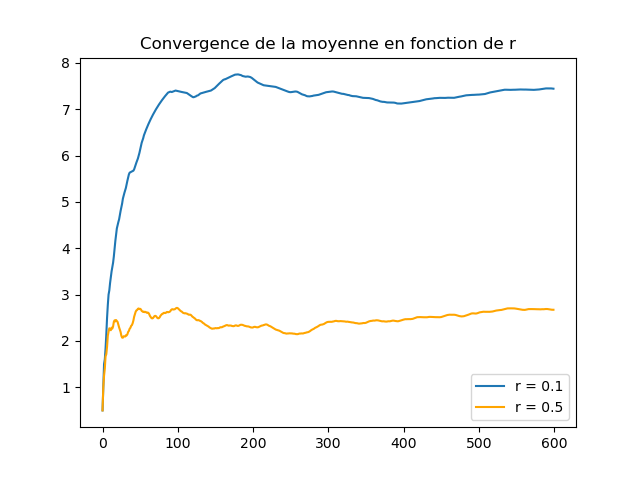
\includegraphics[width=0.5\textwidth]{figs/convergence_mean.png}
  \caption{Convergence de la moyenne pour deux valeurs de $r$}
\end{figure}

\begin{figure}[H]
  \centering
  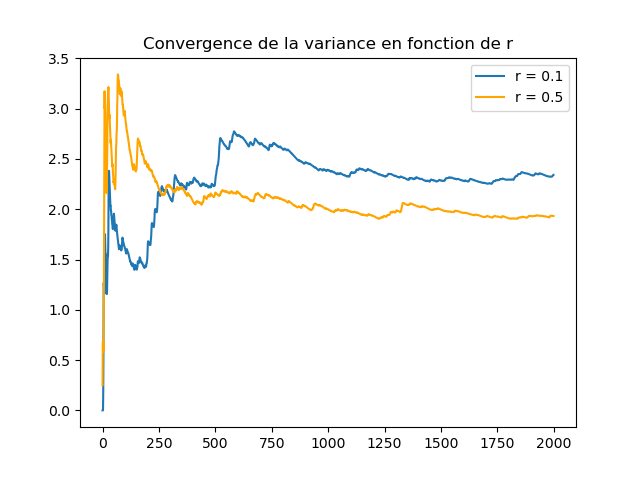
\includegraphics[width=0.5\textwidth]{figs/convergence_var.png}
  \caption{Convergence de la variance pour deux valeurs de $r$}
\end{figure}

Au vu des deux figures ci-dessus, on remarque bien que les valeurs convergent et à des taux différents en fonction de $r$. En effet, plus $r$ est grand, plus on converge rapidement et ce car 
plus $r$ grandit, plus la proportion du cas $0 \leq x \leq K \text{ et } y = x-1$ va prendre de l'importance dans notre distribution, ce qui provoquera une convergence. 

\subsubsection{}
On réalise des histogrammes des fréquences d'apparition pour les deux valeurs de $r$ :

\begin{figure}[!h]
  \centering
  \begin{minipage}{.5\textwidth}
    \centering
    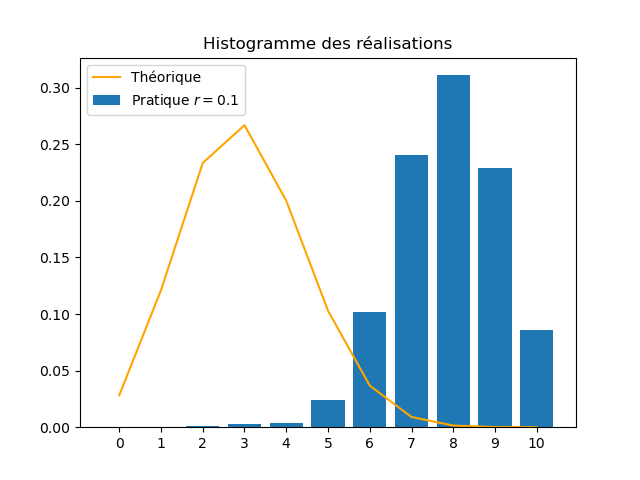
\includegraphics[width=\linewidth]{figs/histo1.png}
    \caption{A figure}
    \label{fig:test1}
  \end{minipage}%
  \begin{minipage}{.5\textwidth}
    \centering
    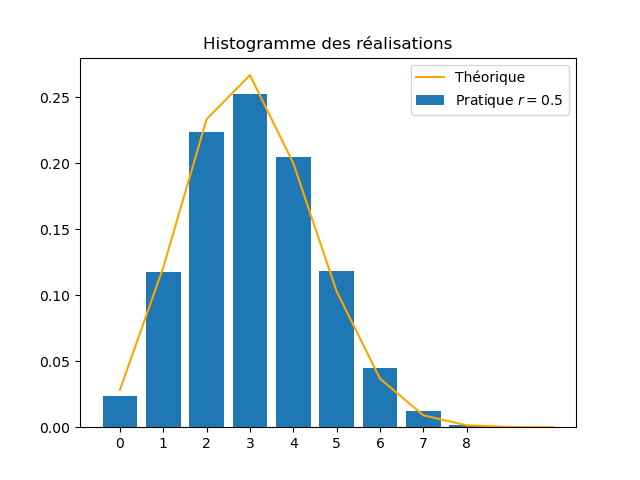
\includegraphics[width=\linewidth]{figs/histo2.png}
    \caption{Another figure}
    \label{fig:test2}
  \end{minipage}
\end{figure}

En comparant les résultats obtenus avec les figures obtenues à la section \ref{section:1.3.2}, on remarque bien qu'on converge vers les mêmes valeurs de moyenne et de variance. Par contre, 
en comparant ces mêmes résultats avec la distribution théorique, on remarque que un des $r$ est beaucoup plus adapté à nos calculs. En effet, dans le cas où $r = 0.5$, nos fréquences d'apparition 
convergent bien vers les valeurs attendues par la distribution théorique.